%!TEX root = ../main.tex

\section{Introduction}
\label{sec:introduction}

3D scanning has gained a lot of interest over the last decades, with methods allowing to reconstruct high quality surfaces from point clouds.
Nowadays, those point clouds are consituted of hundreds of million of points, even just in a single scan.
Acquired surfaces are generally oversampled, and manipulating such amount of data becomes a challenging problem, even just for direct visualization.
Hence, efficient simplification of such data becomes compulsory in order be correctly managed.

\section{Related work}
\label{sec:related_work}

To solve the interactive visualization and compression problems of highly detailed meshes, one common approach considered consists in modifying the connectivity of the reconstructed mesh, to obtain a progressive representation of the surface, that will be refined or coarsened depending on the point of view of the observer in the scene visualized.
To do so, a category of methods consists into a re-triangulation of the mesh, in order to obtain an \textit{implicit subdivision connectivity}. 
After obtaining a coarse approximation of an original mesh, which is called the base mesh, triangles of this mesh are recursively subdivided and newly inserted points are projected onto the surface.
The obtained connectivity is implicit in the way that the only connectivity to store for the whole mesh is the one of the base mesh, the rest of the connectivity is obtained by a recursive subdivision of the triangles.
A survey has recently been done to categorize the different semi-regular remeshing methods in \cite{PRS15}.

Such representation is really suitable for compression purposes \cite{MLDH15} and gained a lot of attractivity over the last years to represent meshes containing a high amount of faces.
However, to obtain such representation, it is necessary add a processing step to the surface reconstruction pipeline, namely \textit{surface remeshing}, with some difficult problems to overcome :
\begin{itemize}
	\item First of all, those methods require most of the time to find a "good" parameterization of the surface, which can be a difficult problem, especially when it comes to handle objects having a really high gender.
	\item Secondly, this introduces a remeshing error between the original mesh and the re-triangulated one, because the new triangulation won't approximate as well the surface acquired.
	\item Finally, this has a certain cost in processing time, which can be non-negligible, especially concerning high-resolution meshes.
\end{itemize}

Considering all of those aspects, we oriented our work into reconstructing a semi-regular mesh directly from the acquired data.

Many 3D acquisition devices do not only provide a 3D point cloud at the output of an acquisition. 
They can also provide 2D parameterizations of a scene from the point of view of a scanner during the acquisition process, in the form of a depthmap (Figure \ref{fig:depthmap_point_cloud}(a)).

Depthmaps are 2D images, where the intensity of each pixel represent the distance of a point in the scene acquired.
Due to the way 3D scanners acquire 3D scenesThis particular structure offers a natural connectivity through the point cloud, where neighboring pixels represent neighboring points on the acquired surface.
Taking this information in consideration, it seems natural to consider this connectivity when it comes to reconstruct the surface underlying the point cloud. 
In this method, we show a method to reconstruct a progressive surface, taking as an input a depthmap and a parametrization function, and producing a semi-regular mesh.
The particularities of the method is that every step is applied in the parametric domain, which simplifies most of the algorithms applied, and the surface is only embed in 3D at the end of the algorithm, using the associated parametrization function.

\begin{figure}[ht]
\centering
\includegraphics[scale=0.05]{DepthMap-Garuda}
\centering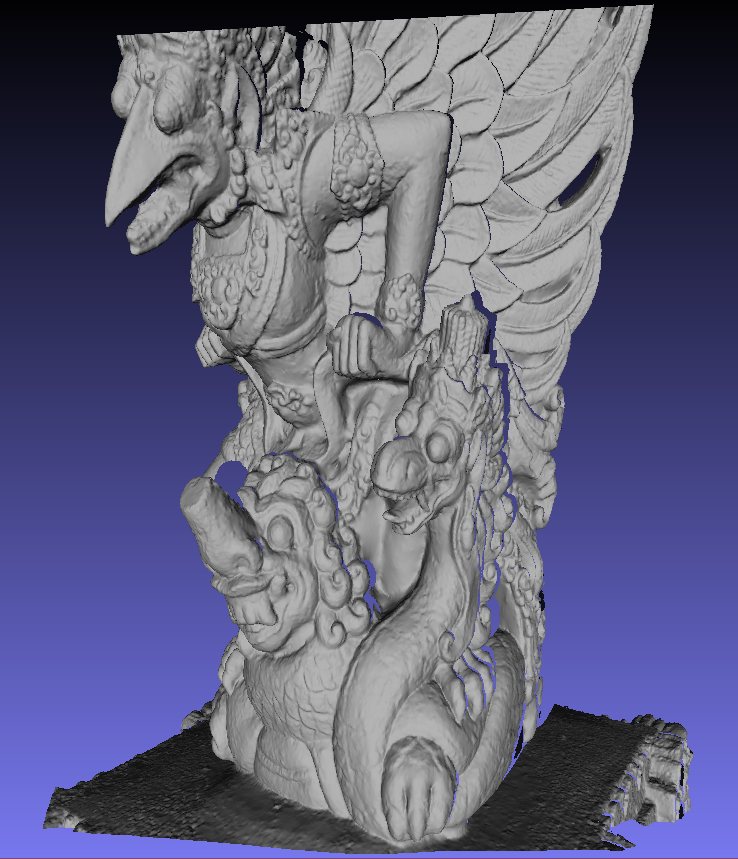
\includegraphics[scale=0.12]{PointCloud-Garuda}
\caption{Example of a depthmap (a) (darker colors represent closer points to the scanner) and the point cloud representing the embedding of the depthmap in 3D (b) (normals have been computed to enhance the visualization).}
\label{fig:depthmap_point_cloud}
\end{figure}

\section{General overview}
\label{sec:general_overview}

Figure \ref{fig:general_steps} represents the different steps of our method used to reconstruct a semi-regular surface mesh from a depthmap.

\begin{figure}[ht]
\centering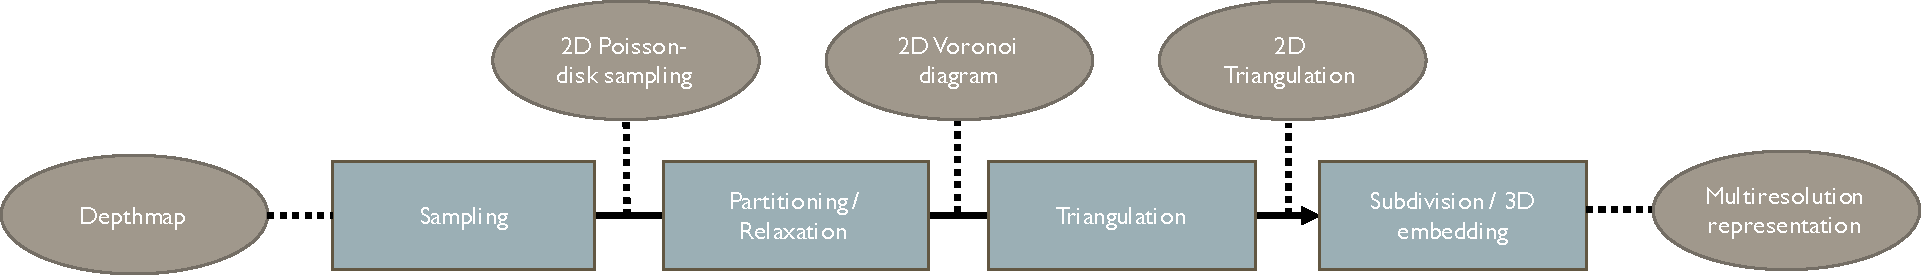
\includegraphics[scale=0.46]{MethodPipeline}
\caption{General steps of our algorithm}
\label{fig:general_steps}
\end{figure}

A priori to everything, borders are detected to identify depth discontinuities (separating 2 surface areas in 3D) and each border is labeled independently.
A Poisson-disk sampling is applied on the depthmap (Section \ref{sec:poisson_sampling}) that will generate the initial sites for a Lloyd relaxation procedure (Section \ref{sec:lloyd_relaxation}). 
Then the obtained Voronoi diagram will be transformed into a 2D triangulation, considering an altered dual representation (taking into account parts identified of the depthmap where two neighboring pixels represent points on different surface areas (Section \ref{sec:border_marking})). 
Finally, from this 2D triangulation, different levels of resolution are reconstructed using a 1-to-4 face subdivision approach (Section \ref{sec:surface_subdivision}).
Finally the reconstructed surface is obtained by embedding the different 2D triangulations obtained in 3D.